\documentclass{article}

\title{Homework 5}
\author{Kelsey Iafrate}
\usepackage{geometry}

\geometry{margin = 1in}

\usepackage{Sweave}
\begin{document}

\maketitle

\Sconcordance{concordance:Homework6.tex:Homework6.Rnw:%
1 8 1 1 0 9 1 1 2 1 0 3 1 12 0 1 2 2 1 1 2 4 0 1 2 34 1 1 2 1 0 2 1 4 0 %
1 2 28 1 1 2 1 0 3 1 12 0 1 2 4 1 1 2 1 0 1 1 11 0 1 2 4 1 1 2 1 0 1 1 %
10 0 1 2 4 1 1 2 1 0 1 1 4 0 1 2 7 1}


\begin{enumerate}

\item

\begin{Schunk}
\begin{Sinput}
> bacteria <- read.csv("~/Documents/Stat103/Data Sets/Bacteria.csv", header=TRUE)
> attach(bacteria)
> fit3 <- aov(Bacteria~Beach*Location)
> summary(fit3)
\end{Sinput}
\begin{Soutput}
               Df Sum Sq Mean Sq F value   Pr(>F)    
Beach           2  364.8   182.4  18.038  0.00071 ***
Location        2 1430.1   715.1  70.720 3.13e-06 ***
Beach:Location  4   57.2    14.3   1.415  0.30471    
Residuals       9   91.0    10.1                     
---
Signif. codes:  0 ‘***’ 0.001 ‘**’ 0.01 ‘*’ 0.05 ‘.’ 0.1 ‘ ’ 1
\end{Soutput}
\end{Schunk}

Since there is not evidence for interaction we should take them out of the model. Values in a and b are for updated model. The decision, however, is unchanged.

\begin{Schunk}
\begin{Sinput}
> fit <- aov(Bacteria~Beach+Location)
\end{Sinput}
\end{Schunk}

\begin{enumerate}

\item

$H_0$: There is no difference in amount of bacteria between types of beaches

$H_A$: There is a difference between some beaches

P-value: 0.000313

Decision: Reject the null. There is significant evidence there is some difference between bacteria levels at some beaches

\item

$H_0$: There is no difference in amount of bacteria between different locations.

$H_A$: There is a difference in levels of bacteria between some locations.

P-value: 2.1e-07 (i.e. super close to zero)

Decision: Reject the null, there are differences in bacteria level between some beaches.

\item

$H_0$: There is no difference in bacteria levels between treatments.

$H_A$: There is a difference in bacteria levels between some treatments.

P-value: 0.30471

Decision: Fail to reject the null hypothesis. We cannot conclude there is any difference between treatments.

\item

\begin{Schunk}
\begin{Sinput}
> par(mfrow = c(1,2), pin = c(2,3), cex = 0.7)
> plot(TukeyHSD(fit,"Beach"))
> plot(TukeyHSD(fit, "Location"))
\end{Sinput}
\end{Schunk}
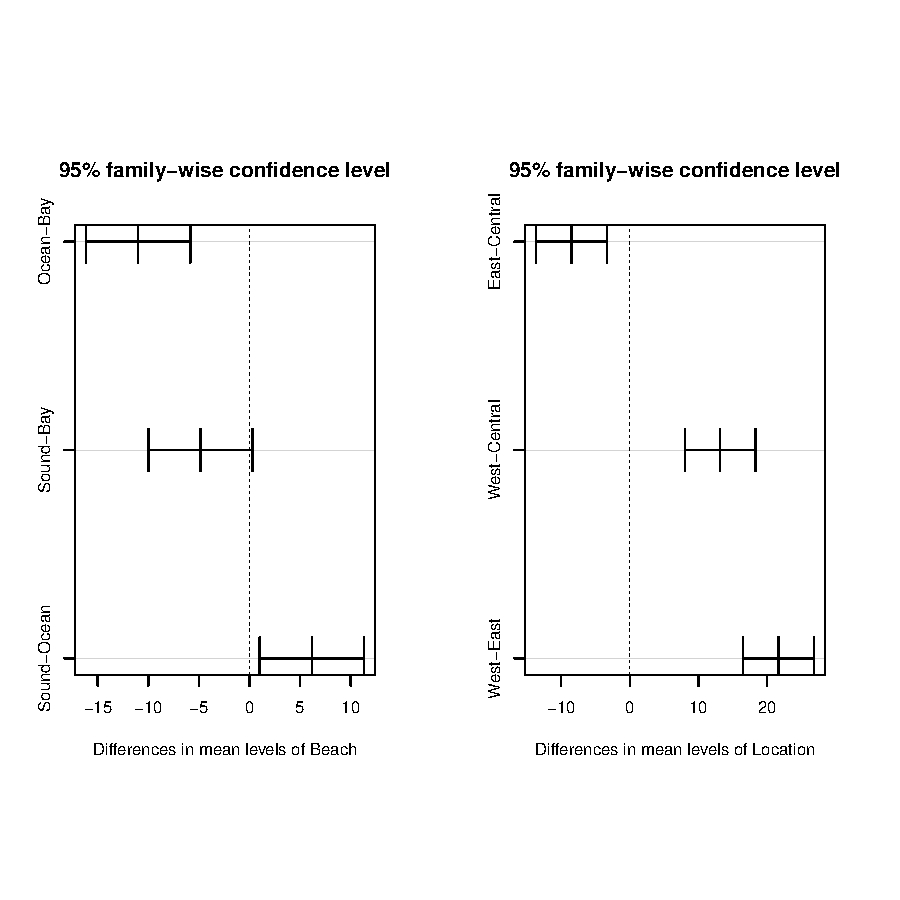
\includegraphics{Homework6-003}

The plots in R are different than stat graphics. For some reason the command to plot the confidence intervals doesn't work, and we saw in my homework 5. The TukeyHSD command gives intervals for the differences. So if the interval does not capture 0, we can conclude there is a significant difference in means between the two factors. 

From the first graph above we can see the difference between the sound and bay is not significant, but the ocean has significantly fewer bacteria on average that both the sound and bay.

From the second graph, we see none of the intervals capture zero, so every difference is significant. So Eastern beaches have the fewest bacteria and Western beaches have the most bacteria, with Central being between the two. 

\end{enumerate}

\item

\begin{enumerate}

\item

The response variable is repair time in minutes.

\item

The factors are the service center number and the brand.

\item

For service center there are levels 1, 2, and 3.

For brand there are Toshiba, Panasonic, and Sony.

\item

\begin{Schunk}
\begin{Sinput}
> VCR <- read.csv("~/Documents/Stat103/Data Sets/VCR.csv", header=TRUE)
> attach(VCR)
> timeFit <- aov(Time~Center*Brand)
> summary(timeFit)
\end{Sinput}
\begin{Soutput}
             Df Sum Sq Mean Sq F value  Pr(>F)   
Center        1   24.1    24.1   0.691 0.42216   
Brand         2  901.3   450.7  12.925 0.00102 **
Center:Brand  2  260.2   130.1   3.731 0.05496 . 
Residuals    12  418.4    34.9                   
---
Signif. codes:  0 ‘***’ 0.001 ‘**’ 0.01 ‘*’ 0.05 ‘.’ 0.1 ‘ ’ 1
\end{Soutput}
\end{Schunk}

There is not significant evidence that there is a interaction due to service center and VCR brand.

\item

\begin{Schunk}
\begin{Sinput}
> timeFit2 <- aov(Time ~ Center+Brand)
> summary(timeFit2)
\end{Sinput}
\begin{Soutput}
            Df Sum Sq Mean Sq F value Pr(>F)   
Center       1   24.1    24.1   0.497 0.4924   
Brand        2  901.3   450.7   9.298 0.0027 **
Residuals   14  678.6    48.5                  
---
Signif. codes:  0 ‘***’ 0.001 ‘**’ 0.01 ‘*’ 0.05 ‘.’ 0.1 ‘ ’ 1
\end{Soutput}
\end{Schunk}

There is not enough evidence to claim there is an effect due to service centers.

\item

\begin{Schunk}
\begin{Sinput}
> timeFit3 <- aov(Time~Brand)
> summary(timeFit3)
\end{Sinput}
\begin{Soutput}
            Df Sum Sq Mean Sq F value  Pr(>F)   
Brand        2  901.3   450.7    9.62 0.00205 **
Residuals   15  702.7    46.8                   
---
Signif. codes:  0 ‘***’ 0.001 ‘**’ 0.01 ‘*’ 0.05 ‘.’ 0.1 ‘ ’ 1
\end{Soutput}
\end{Schunk}

There is an effect on repair time due to VCR brand since the P-value is 0.002049.

\item

\begin{Schunk}
\begin{Sinput}
> par(pin=c(4,3), cex = 0.8)
> plot(TukeyHSD(timeFit3))
\end{Sinput}
\end{Schunk}
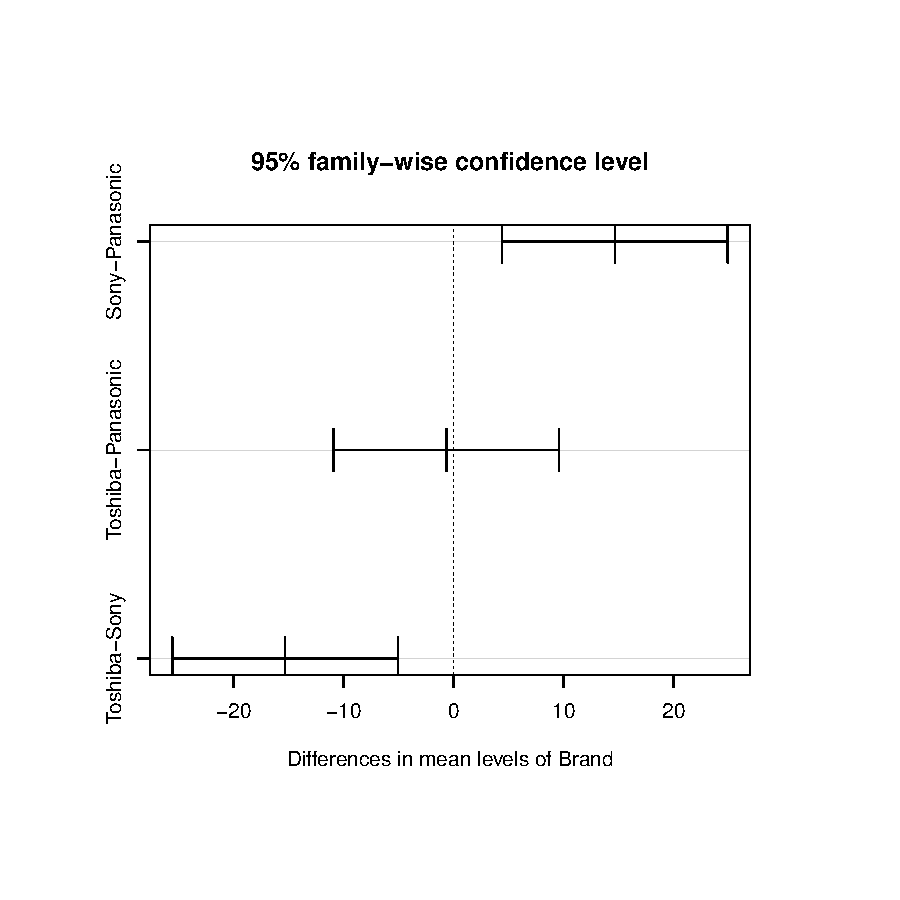
\includegraphics{Homework6-007}

The service should conclude that Sony decisively has the highest repair time, and that there is not statistical significance between Toshiba and Panasonic. 

\end{enumerate}

\end{enumerate}

\end{document}
